
\section{Aula 6.2 - Modulação M-PAM}

O objetivo desta aula é demonstrar uma técnica alternativa de modulação de sinal digital a modulação M-PAM, aqui constrastaremos a mesma com a alternativa PCM, conceitualmente
o que a difere da previamente mencionada e porque ou não usar uma ou a outra.
\\

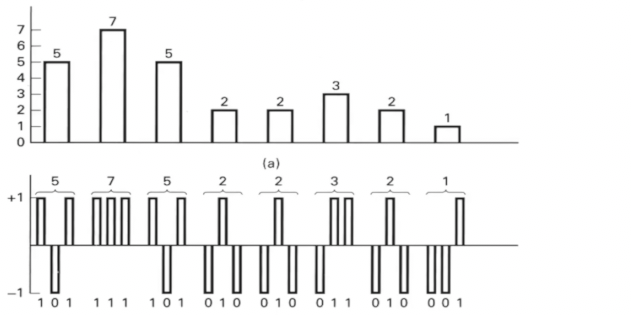
\includegraphics[width=0.7\textwidth]{../assets/mpam.png}

\subsection{O que é a modulação PCM mesmo?}

Lembrando do diagrama de comunicação:


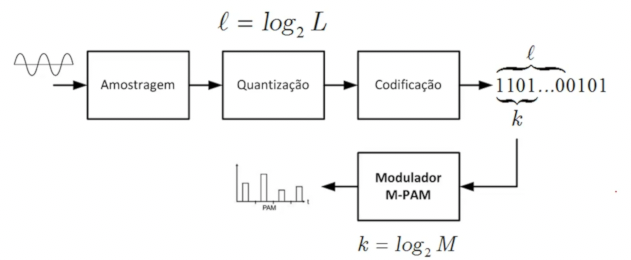
\includegraphics[width=0.6\textwidth]{../assets/diagramacomm.png}


Note que o sinal é amostrado isto é a uma dada frequência o valor atual do sinal é capturado e enviado para um conversor ADC,analógico digital, na saída obtemos o sinal quantizado
que é pegar os possíveis valores do sinal analógico, os limites, e associar uma sequência de bits que melhor mapeie aquele nível lógico, note que quanto mais bits mais preciso,
porém mais caro, depois é a etapa de codificação que faz o mapeamento daquela sequência de bits em uma segunda sequência de bits denominada \textbf{símbolos} e agora é onde entra
a modulação PCM, cada símbolo é composto de k bits a modulação PCM envia k bits numa transição de maneira individualizada, cada bit é enviado em frações do período para transição
de forma que é necessário examinar k bits para saber o símbolo transmitido.

\subsection{Porque então a modulação M-PAM?}

Note que há uma escolha na etapa de modulação, é possível fazer um terceiro mapeamento dos k bits em níveis discretos de amplitude, então suponha que um exemplo de k bits
fosse 101 isso seria mapeado no nível de amplitude 5, visto que 000 seria mapeado no 0 de nível de amplitude e 111 seria mapeado em 7 de nível de amplitude, logo diminuindo
o número de bits transmitido efetivamente diminui a largura de banda e essa é a maior vantagem dessa modulação, note no entanto que na velocidade de informação é essencialmente
a mesma visto que tal modulação não comprime o tempo de envio e portanto o tempo para chegar os k bits que representam o símbolo na modulação PCM é o tempo para chegar o sinal
modulado em amplitude.

\subsection{Comparando as abordagens, não há bala de prata \emoji{😢}}

E novamente voltamos a velha tautologia conhecida pelos engenheiros, não há solução perfeita. Ora o que a modulação M-PAM nos fornece é ótimo, mas o gasto de potência é muito maior
visto que não só o transmissor como o receptor precisam modular níveis de amplitudes para o total de símbolos que existam no esquema de comunicação, mas ainda há um outro problema
quanto mais níveis de amplitude maior se torna o problema de detecção simbólica visto que a diferença de níveis de amplitude tende a diminuir e consequenmente erros ficam mais custosos de serem detectados ou até mesmo corrigidos.

\subsection{E não tem equação nessa aula?}

Sim tem uma bastante importante que ajuda a dimensionar a quantidade de bits de acordo com o erro de quantização desejado, lembre-se que indepedente do número de estados para
quantizar a amostra o erro entre estados é no máximo, pior caso, $|e|_{max}=\frac{q}{2}$ e sabendo disso e da seguinte desigualdade: $|e| \le pV_{pp}$ obtemos a relação final:

\begin{equation}
	L \ge \frac{1}{2p}
\end{equation}

\begin{equation}
	l \ge \log_{2}(\frac{1}{2p})
\end{equation}

onde $L=2^{l}$

